
The contradictory conclusions that arise from the experimental results presented in Figure~\ref{fig:BestWorstComparison} are caused by two issues: (1) the representation of a space of program behaviours by a single point in that space; and (2) the modelling of the effect of uncontrolled variables on the result of the experiments. The use of \CP\ with a leave-one-out evaluation methodology leads to a more appropriate evaluation of the space of behaviour variations due to data input. The repetition of each experiment a reasonable number of times and the reporting of the average of these runs with a corresponding confidence interval to inform about this variation leads to a better accounting for he effect of uncontrolled variables that affect the results of the experiments. The result is a more accurate prediction of performance from the benchmark-based evaluation.

\REM{
This section explains the issues of collecting and analyzing data in the experimental setting. To have a minimum amount of confidence in the values collected it is mandatory to have a strong knowledge of the environment, how much noise could the data possibly have, and how to overcome the difficulties in the measuring process. There is a method to follow and then make sure the data analysis is correct and sound. At first, there is always noise, but the level of the noise will have impact on the number of times an experiment must be repeated; second, after collecting the data the analysis must be carried out, hence as there is noise it is mandatory to show the noise level, showing the values through the use of error bars (for the variance found in the data). Nonetheless this section uses these variance to explain the speedup and slowdown results of \refSection{sec:speedup}.

Every experimental science suffer from the same problem, evaluation of the data already collected. Even the simple idea of collecting data can become a painful task, because the measurement process may introduce errors, or cause distortion in the data.
}

Uncontrolled variables include processes running in background, operating system calls, interruptions, memory allocation, and other sources, including the measurement process itself. Hence, it is important to have a good understanding of the sources of performance disturbances in  the system~\cite{Kalibera2013}.
Kalibera and Jones state that the majority of the experimental studies lack a rigorous statistical methodology~ \cite{Kalibera2013}. A methodology to deal with the effect of uncontrolled variables is to examine the distribution of the data and identify measurements that can safely be eliminated because they are tainted by the effect of uncontrolled variables. For instance, \refFigure{fig:gauss} depicts a scatter plot of $1000$ runs of the program \bzip\  compiled using the \funcname{Static} inliner (\llvm) and run with the {\tt ebooks} input. Each poin in the scatter plot represents the running time for a single run and the runs are ordered in the horizontal axis according to the order in which they were executed. For \bzip\ and \gzip\ the code used is not the one distributed by SPEC, but rather fully-functional versions of these programs. Using these versions eliminates the unrealistically-simplified profiling situation where mutually-exclusive use cases are combined into a single program run. Consequently, these programs cannot do decompression and compression, or multiple levels of compression, within the same run.  These distinct use-cases must be covered by different inputs in the program workload.
The inputs for compression include images, ebooks in a variety of formats, movies in MP4 format, textual representation of proteins, audio books, and object files~\cite{BerubePhD}.

\refFigure{fig:gauss} reveals a gaussian noise around the median plus some outliers that are the result of regular operating system activity. These outliers can safely be filtered out from the data set. They are easily discarded because they are more than one standard deviation above the median. similar plots for other benchmarks --- not shown --- revealed that the distribution of execution time follows a similar pattern with outliers that can be easily filterred out.

\jna{Make fonts much bigger in \refFigure{fig:gauss}, also change "runs" to "run" in the horizontal axis because "runs" could be the number of runs represented by a point.}
\rlar{The scatter plots were generated by Matlab, I am trying to correct this one, but I'm not being successful. Probably the connection, or the server, are overloaded today, I'll have to try again later.}
\begin{figure}
  \centering
  \includegraphics[width=1.00\linewidth]{Figures/nt1000}
  \caption{Scatter plot of the execution times from $1000$ runs of \bzip\ with {\tt ebooks} data input. The execution times appear in the graph in the order in which they were measured.}
  \label{fig:gauss}
\end{figure}

\jna{Are the three independent experiments also runs of \bzip\ with {\tt ebooks} or are they something else? We need to be specific about which benchmark was run with which input.}
\rlar{Yes, these three independent experiments are also runs of \bzip with {\tt ebooks}, the idea behind it was to compare the means and noise between them, 10X100, 10X1000, 100X1000. Written below.}
Three independent experiments also running \bzip with {\tt ebooks}, with $10$ runs, $100$ runs, and $1000$ runs, reinforces that outliers can be discarded because there is high probability that the measured means have minimum difference among them, and also the behaviour of the program remained unchanged \paul{How do you know the behaviour is the same in the outliers as in the other runs? Same running-time does not imply same behaviour.}. 
Simple statistics --- mean, median, standard-deviation from the mean (std-mean) and standard-deviation from the median (std-median) --- shown in \refTable{tab:robustTest} indicate that the distribution is quite similar for the different number of runs.. \rlar{completed in response to your comment/question}
\jna{Is this the correct interpretation of the result of the t-tests?}
\rlar{As we discussed by email, we only have evidence that the results point to failing to reject the null hypotheses. But there is still a possibility of making a type II error stating that the means are the same. So we can only say that since the null hypothesis is reject there is a probability (based on the p-values) that the means may be same. What you are saying is correct, we cannot state that the means are the same, they have a p-value probability of being the same.}
To improve the confidence that the means have high probability of being the same, t-tests between sample pairs of the three independent distributions were also run. The t-tests were employed to determine if two sample pairs of data sets are significantly different from each other, and the null hypothesis for the t-tests was that the means are the same \paul{Are you comparing the mean of the 10-run date to the mean of the 100-run data to the mean of the 1000-run data?  What would that show? All the data is taken from the same distribution, just the sample sizes are different.  We expect that they'll all have the same mean, particularly as the sample size increases.  If you're trying to show that it's OK to remove outliers, then your experiement needs to be comparing results with and without outliers.  I would have expected that you'd compare 10-runs with outliers to 10-runs without outliers, 100-runs with to 100-runs without, \etc.}. The results point to not discard the null hypothesis, as shown in \refTable{tab:ttest}.

The supposition is that the data follow the normal distribution, and the two-sample t-test were run. The value $0$ are displayed to show that the null hypotheses cannot be discarded, it can also be read as {\tt false} \paul{The meaning of the column should be immediatly evident from the table.  Perhaps rename the column to ``Reject $H_0$?'' and change the 0s to ``no''}. As the p-values are low so the confidence is higher so, even knowing that mistakes can be made, assuming that the distributions tend to be normal the null hypotheses cannot be discarded \paul{The p-values are not low, they are between 0.15 and 0.6.  Aren't we looking for at least $p<\alpha=0.05$ in order to reject the null (95\% confifidence)?  These p-values are too large, so we cannot reject the null...}.

\jna{All the captions for all the tables, and graphs, must be rewritten to much more precisely describe what the tables and figures are showing, saying "Simple statistics on the experiment", "t-tests applied pairwise to the $10$, $100$, and $1000$ runs", "Test on the means", etc, is not very helpful. In a good paper, the reader should be able to look at the figure/table, read the caption, and know what is going on without necessarily reading the text.}
\rlar{Ok, I'll do it later. For now I'm trying to put things in order for you, so you can continue your corrections. I had a hard time trying to edit the files and finding that I couldn't push them because there was a conflict, I hope now everything is fine.}
\begin{table}
  \centering
  \begin{tiny}
  \input{Tables/robustTest}
  \end{tiny}
  \caption{Variation in statistics when the number of experimental runs is changed for <NameOfBenchmark> with <Input>.}
  \label{tab:robustTest}
\end{table}

\jna{We need a clearer and more complete description of the t-tests that were run. Did we run a one-sample or a two-sample t-test? (see http://en.wikipedia.org/wiki/Student's\_t-test). What does the value 0 in all rows of the table mean and how should they be interpreted? Why these p-values prevent us from discarding the null hypothesis? Our logic seems to be that because we did not discard the null hypothesis, we must conclude that the means are similar. Is that a correct reasoning?}
\rlar{We suppose that the distribution is normal, but if the data are substantially non-normal and the sample size is small, the t-test can give misleading results. This is a risk that we are willing to take. We ran the two-sample t-test. About the value 0, they were returned by MatLab to show that the null hypotheses cannot be discarded it can be read as a 'false' as well. The p-values, except for the case 10-1000 are low, so the confidence is higher. In the 10-1000 case the p-value gives us a confidence of less than 40\%. Concerning the logic applied, as mentioned earlier, we can still make mistakes, but we assume that the distributions tend to be normal and we believe that we cannot discard the null hypotheses.}

%The t-tests in \refTable{tab:ttest} demonstrates that the null hypothesis cannot be discarded, as the value $0$ in each line of the \emph{t-test} column confirms, which means that the three means are similar. The \emph{p-values} show the confidence in the hypothesis, in this case that the means are different. As the values are not high, the confidence is very low.

\begin{table}
  \centering
  \begin{tiny}
  
\begin{tabular}{lllll}

{\bf Runs} & {\bf Reject $H_0$} & {\bf p-value}  \\ \hline

(10-100) & No & 0.3424  \\
(10-1000) & No & 0.6025 \\
(100-1000) & No & 0.1528 \\

\hline
\end{tabular}

  \end{tiny}
  \caption{t-tests applied pairwise to the experiments with $10$, $100$, and $1000$ runs of Table~\ref{tab:robustTest}.}
  \label{tab:ttest}
\end{table}

\jna{A main issue that I have with the description of all the experiments in the paper is that these descriptions are not specific enough. They don't tell me which benchmark program was used, which inputs, etc. For example in the paragraph below: (1)
What "running the same data" means? Is it executing the same version of the benchmark with the same input? (2) What "is not quite different"? Can we give a numerical value that is the basis for this statement? (3) What is an 'input-run' and why are we using single quotes when we mention it? (4) What "the whole experiment" means? (5) What is a 'full-run'? (6) What 'by the end of the experiment' mean? Is it the case that the noise was added to the measured values after the experiment was completed?}
\rlar{I tried to rewrite the paragraphs below, but I don`t know if they describe what we need as they are now.}

After running the experiments on \bzip with {\tt ebooks} as input and observing no relevant difference on the means, the next step was to define the minimum number of times a program has to be run to produce reliable data. An experiment was devised to account for this question, the main idea was to increase the number of times a program had to run starting from $3$ times until $10$ times, because the former experiment had already set the last value as reliable \paul{From this sentence, I think you're going to run the experiement, using [3..10] runs on an input, and averaging those to measure the running time on that input.}. So the experiment used the benchmarks for \bzip, \gzip, \gcc, \gobmk applying all inputs, but each input was run $3$ consecutive times \paul{But now you say you only ever used 3 runs}. After running a program with all inputs $3$ consecutive times, the same program was run again repeating the same experiment $100$ times \paul{How does re-running the 3-run experiment relate to your stated goal of finding out how many runs are needed?}. In total each input was run $300$ times, but the whole experiment was run $100$ times, and each input was exercised $3$ consecutive times at each experiment.

The complete experiment included some extra noise, simulating an `uncontrolled variable' \cite{Kalibera2013}, caused by the execution in parallel on the same machines of a copy of the system \paul{Wait, what?  Now you're adding noise and trying to figure out how many runs are needed at the same time?  Shouldn't these be two separate experiemnts?}. The purpose was to stress the system and compare the behaviour with noise and without noise \paul{That definitely sounds like a different experiment}. The noise was added after $75$ of the $100$ runs of the experiment, increasing the running time of the programs, as expected. But the deviation from the mean is not large in the segment with noise, as shown in \refFigure{fig:CProbust}. The figure depicts data for program \bzip running with input {\tt ebooks}. The running time for the program at each $3$ consecutive run can be found on the $y$-axis of \refFigure{CP:ebooks}, and the order number is depicted on the $x$-axis \paul{I don't know how to read the figure or how it supports your claim.  What does a single point represent?  Why are there those really high outliers, and what does that mean in terms of the claims you're trying to make?  Why is there a large spike at 230?  If that's where you added noise, why does it go away?  If there is a point on the figure where noise is added, it would be nice if there was a vertical line to mark that point.}.

The extra noise can be easily visualized as the histogram \refFigure{CP:hist}, where the $x$-axis depicts the running time for the program and the $y$-axis depicts the number of runs at each bin \paul{The caption says 'auriel'... is the caption wrong, or is this different data?  I see at least 4 points in part a that are above 8.9, but that isn't even in range of your histogram.  How does the histogram visualize the noise? The x-axis labels don't match up with the histogram bins. All I see is a distribution... there is no distinction between data from noisy and non-noisy systems}. The two figures of refFigure{fig:CProbust} show the $3$-consecutive run for \bzip having {\tt ebooks} as input data. The running time of the program was increased on the bins where the noise is present, but the behaviour of the system kept the same pattern, showing that it is robust \paul{What pattern? You haven't said anything about a pattern, and a running-time isn't a pattern.  If you want to talk about patterns of behaviour, I expect to see a figure (and a matching analysis) like those in phase-profiling papers}.

%Another experiment has also shown that the variance when running the same data just three times in a row is not quite different from the one running $100$ times. This experiment was constructed by exercising each `input-run' $3$ times, $3$-consecutive runs for each input, and the whole experiment was run $100$ times% -- which means that the experiment ran $300$ times each input.
%A `full-run' in this experiment is a $3$-consecutive run for each input, hence the experiment ran $100$ `full-runs'. Nevertheless the behavior of the system was stressed through the addition of extra noise, simulating an `uncontrolled variable' \cite{Kalibera2013}. The extra noise was injected by the end of the experiment.

\jna{What is this "subtle knob"? This "knob" has to be precisely described. This "another system" must be precisely specified? What exactly was running at the same time?}
\rlar{Answered on paragraphs above.}
%The purpose of the extra noise was to verify if the system was robust, even though the effect of the noise can mask the correct values, these data can treated assuring robustness. This way the \CP\ methodology was empirically verified with respect to soundness. As can be seen in \refFigure{fig:CProbust}, the deviation from the mean is not large, and also that there is a subtle knob, which increases the running time of the all programs. It was caused by the execution of another system at the same time competing for the same resources. The running time of each program at each 3-consecutive run can be found in the $y$-axis of \refFigure{CP:ebooks}, and the order number of each full-run is depicted on the $x$-axis. The extra noise can also be visualized in the histogram of \refFigure{CP:hist}, where the $x$-axis depicts the running time for the program and the $y$-axis depicts the number of runs at each bin. These two figures show the $3$-consecutive run for the input data {\tt ebooks}.

\begin{figure}
  \centering
  \begin{minipage}[t]{\linewidth}
    \subfigure[$100$-time runs of the $3$-consecutive execution of input {\tt ebooks} for program \bzip] {
      \begin{minipage}[b]{0.75\textwidth}
        \centering
        \includegraphics[height=12em]{Figures/ebooks300}
      \end{minipage}
      \label{CP:ebooks}
    }
    \vspace{1em}
    \hrule
    \vspace{1em}
    \subfigure[Histogram for the {\tt auriel} input] {
      \begin{minipage}[b]{0.75\textwidth}
        \centering
        \includegraphics[height=12em]{Figures/ebooks}
      \end{minipage}
      \label{CP:hist}
    }
  \end{minipage}
  \caption{$100$-times running $3$-consecutive experiment}
  \label{fig:CProbust}
\end{figure}

What these two experiments, shown in \refFigure{fig:CProbust} and \refFigure{fig:gauss}, strongly tell is that collecting data from single execution can produce erroneous results, even using machines with no other running program. And this happens because of the very nature of the empirical experiments, there is some noisy data distribution caused by regular operating system activities, interruption calls, etc. But also, as shown in \refFigure{fig:CProbust}, that these effects can be mitigated by multiple-run experiments. The latter experiment also have shown that in the present case running $3$ consecutive times is enough to acquire robustness.
%\refFigure{fig:CProbust} and \refFigure{fig:gauss} show that collecting data from single execution can produce erroneous results, even using machines with no other running program. This happens because of the very nature of the empirical experiments, there is some noisy data distribution caused by regular operating system activities, interruption calls, etc. Also, an inclusion of a simple task during the running cycle can perturb the execution time of the program under evaluation, as can be observed by the knob in \refFigure{fig:CProbust}.

The data collected from the experiment are shown in \refTable{tab:simStats}, and the deviations from the mean (and median) to each $3$-consecutive run are summarized as the average, minimum, and maximum values. The data shown in this table is from the experiment on \bzip running {\tt ebooks} as input.

\begin{table}
  \centering
  \begin{tiny}
  \input{Tables/simStats}
  \end{tiny}
  \caption{Deviation from the mean and from the median in the experiment}
  \label{tab:simStats}
\end{table}

T-tests were run to confirm that the means are statistically representative of the same distribution. This is summarized in \refTable{tab:statTest} below. It is easy to see that the number of outliers is little, except for the noisy region.
%To confirm that the means are statistically representing the same distribution the t-tests were also run. This is summarized in \refTable{tab:statTest} below. It is easy to see that the number of outliers is little, except for the knob region. 
%because the runtime was being raised during certain amount of time pushing a gradient to increase the time values, and after it, what happened was the other way around, decreasing the time values. Both tables \refTable{tab:simStats} and \refTable{tab:statTest} are shown for the runs.

\begin{table}
  \centering
  \begin{tiny}
  \input{Tables/statTest}
  \end{tiny}
  \caption{Test on the means}
  \label{tab:statTest}
\end{table}

%This kind of experiment can bring confidence in the data collected. In our case it brought confidence in the machine learning method devised to tune-in the inlining parameters of the compiler. 
To obtain low variance one possibility is to increase the number of consecutive runs for each individual input. Nevertheless, these experiments have shown that $3$-consecutive run is a good choice, because it does not penalize much the total running time of the system.

The experiments also have shown that single-run testbeds are error-prone because they don't take the variance into account. The results of an experiment (speedups, or slowdowns) are robust only if there is statistical assurance that the variance on the data is not large.


\section{The Actual Performance Variations}

The complete and correct values are described below. $18$ different settings were structured for \bzip\ and $20$ for \gzip, employing the same setup (hardware and software) and the data from each input were collected in these settings. The purpose of these experiments were to establish the variance a researcher could find running the experiment on different, but similar, machines, and doing so to show that single-run experiments can lead to erroneous results. This section ends with a figure that was generated by the \CP\ framework, where the error bars are clearly depicted in it, showing the variance on the speedup geometric means.

\subsubsection{Analysis of\ \ \bzip\  and  \gzip}

After analyzing the inlining environment and having the confidence that the results are trustful, the first program studied was \bzip. 
\jna{What are these 18 settings? Have we described them before? How did we arrive at 18 of them? --- As a reader I would not really know what is going on. See Berube's Ph.D. thesis to learn that Never does not mean no inlining! What does "collecting data" means? I suspect that there are many runs with different sets of training inputs, and testing inputs that goes into the calculation of each point in \refFigure{fig:fdllrep}. We need to explain this process.}
\rlar{The settings are explained above. About Never, the original intent is to avoid inlining, but when the thesis was written it was not actually working this way, but it was corrected later and is working this way, no inlining is performed. About the data collected, they refer to the runtime of each input exercised, and all inputs were used.}
%Collecting data from the same setup (hardware and software) in $18$ different settings was the first step. 
\refFigure{fig:fdllrep} shows the data collected. The vertical axis shows the normalized execution geometric mean time for each setting, the baseline is Never (no inlining), and the horizontal axis shows the settings organized by number. The red ``*" represent the normalized geomean time of the \FDI\ inlined program, and the blue ``o" represent the normalized geomean for \llvm\ inlined program.

\begin{figure}
  \centering
  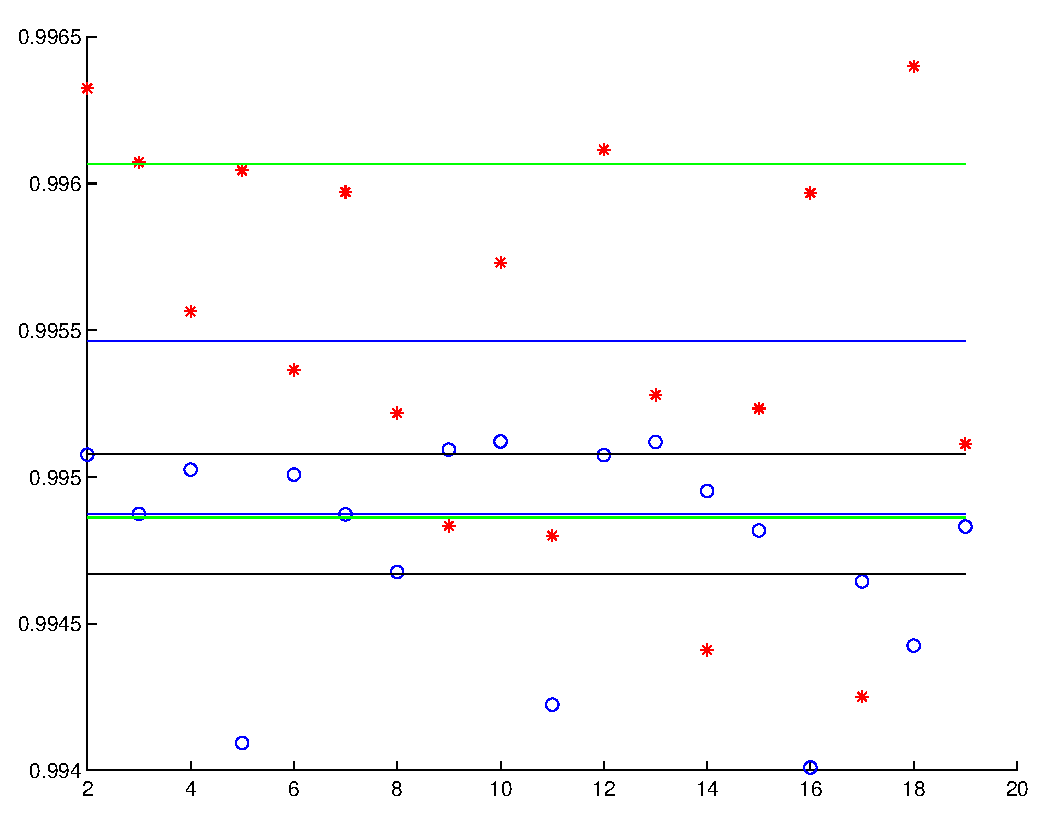
\includegraphics[width=1.00\linewidth]{Figures/fdllrep}
  \caption{The $18$ different settings for \bzip\ of the same setup}
  \label{fig:fdllrep}
\end{figure}

The blue lines in the figure show each median value for the geometric means, the green lines represent one standard deviation from the median for the \FDI\ case, while the black lines represent the standard deviation from the median for the \llvm\ case. As it can be seen, not only the values are too similar, varying only from the fourth decimal digit, but also the medians and their standard deviations overlap, collapse. This is a strong indicator that there is no significant difference between those measures.

Just consider that a single-run experiment could have measured any one of the $3$-consecutive run values individually, moreover, a single run may have also collected the best, or the worst values for the actual times of the experiment. Hence, one experiment using a single-run methodology could produce a speedup for \FDI\ if the experiment by chance had collected the worst running time for \llvm\ inlined program, and the best running time for the \FDI\ inlined program.

\jna{What is the justification for this "adjusting" the data? Is there a plausible real-life situation where a well-meaning scientist would end up doing such adjustment? --- either on purpose or by mistake?}
\rlar{Yes, this is our main claim, a scientist using a single-run methodology could gather the "adjusted" data, for a speedup or a slowdown. And this is what the last paragraph was trying to state, I have rewritten part of it. About the input set, the text does not reflect what was shown in the section, there was no adjusting.}

Consider the case where some input data could not be run because the environment and the complexity of the experiment break the program when executing these inputs. In this case the researcher would have to report the data with missing values, and also to tell that there are some missing values due to some execution problems. Suppose that these inputs were exactly the ones that produced slowdowns, or tiny speedups, in this case a bigger speedup could have been observed. Now, using the data collected in the experiment the speedup was only of $0.46 \%$, but if some input data could not be gathered, especially the slowdowns and some of the tiny speedups, the value for the speedup could have grown. The data for the complete experiment producing the speedup are shown in table \refTable{tab:fullexp}.
%Even though this biased data showed a speedup, it was really worthless, only $0.46 \%$. Therefore, to reinforce that the input set is also a big issue, the data were "adjusted", leaving the slowdowns and some of the tiny speedups gathered from the set of inputs out of the final list to be shown. This way a tiny, but possibly measurable speedup, was presented in \refSection{sec:speedup}. Nevertheless, defining a list of inputs is an issue and has to be treated as part of the experiment design, as this ``speedup'' have shown. The full data for the "speedup" experiment are shown in table \refTable{tab:fullexp}.

\begin{table}
  \centering
  \begin{tiny}
  
\begin{tabular}{lllll}

{\bf Input} & {\bf Normalized \FDO} & {\bf Normalized \llvm} & {\bf Speedup} \\ \hline

auriel & 0.9720 & 1.0076 & 0.9647   \\ 
avernum & 0.9922 & 0.9905 & 1.0017 \\
cards & 0.9909 & 0.9989 & 0.9919  \\
ebooks & 0.9909 & 0.9920 & 0.9988  \\
gcc & 0.9966 & 1.0059 & 0.9907  \\ 
lib-a & 0.9940 & 0.9970 & 0.9970  \\ 
mohicans & 1.0000 & 1.0048 & 0.9951  \\
ocal & 0.9988 &1.0075 & 0.9913  \\ 
paintings & 1.0000 & 1.0051 & 0.9949  \\
potemkin & 0.9916 & 0.9887 & 1.0029  \\
proteins-1 & 0.9977 & 0.9910 & 1.0068  \\
proteins-2 & 0.9813 & 0.9950 & 0.9862  \\
revelation & 0.9868 & 0.9887 & 0.9980  \\ 
sherlock & 1.0000 & 1.0020 &1.0125  \\ 
usrlib & 1.0000 & 0.9875& 1.0458  \\  \hline
Speedup & & & 0.9953 (0.46 \%) \\

\hline
\end{tabular}

  \end{tiny}
  \caption{Summary of the normalized data used to produce a speedup for \bzip}
  \label{tab:fullexp}
\end{table}

In \refSection{sec:slowdown} a slowdown was shown. This slowdown could have also been generated if a single-run methodology were employed, because the experiment could have gathered the worst individual running time for the \FDI\ inlined program and the best running time for the \llvm\ inlined program. This way a different measure, using the same infrastructure could produce a slowdown instead of a speedup. And as both results followed the same methodology, they are both correct, and this is unexplainable unless considering that there is variance on the data collected.
%On the other hand, in \refSection{sec:slowdown} the opposite was performed, choosing the worst individual running time for the \FDI\ inlined program and the best running time for the \llvm\ inlined program. Proceeding this way it was easy to present, from "a different" individual measuring, a slowdown. And as both results followed the same methodology, they are both correct, and this is unexplainable unless considering that there is variance on the data collected.

The same process was employed for the \gzip\ case, using $20$ different settings. \refFigure{fig:gzipfdll} presents the \gzip\ data in the same way of \refFigure{fig:fdllrep}. From \refFigure{fig:gzipfdll} there can be seen no evidence of speedup for this setup, and even though, a speedup could have been reported.

\begin{figure}
  \centering
  \includegraphics[width=1.00\linewidth]{Figures/gzipfdll}
  \caption{The $20$ different settings for \gzip\ of the same setup}
  \label{fig:gzipfdll}
\end{figure}

Although these cases were artificially constructed from empirical data, if a single-run methodology was employed these results could appear. But employing \CP\ methodology allows a researcher to correctly identify the statistical variance on the data and to discard false speedups or slowdowns. This result, in a certain way, reinforces the result of Curtsinger and Berger, reporting no speedup of $-O2$ over $-O3$ for all benchmarks they analyzed, when code randomization is applied~\cite{Curtsinger2013}.

%=============== GOBMK

\subsubsection{Analysis of \gobmk}

%For \gobmk\ the input set was chosen considering that some of the inputs could have broken the execution cycle of the program, so some inputs were excluded from the set in a similar way to that for \bzip\ and \gzip\ cases. 
The full 15-input set was applied for \gobmk, and for the full input-set the experiment produced a speedup of $1.01 \%$, as shown in \refTable{tab:fullspeedupgbk} and in \refFigure{fig:gobmkall}.

\begin{table}
  \centering
  \begin{tiny}
  
\begin{tabular}{lllll}

{\bf Input} & {\bf \FDO\ normalized} & {\bf \llvm\ normalized} & {\bf Speedup} \\ \hline

13x13 & 0.9922 & 0.9983 & 0.9938  \\
arb & 0.9939 & 0.9969 & 0.9969  \\
arend & 0.9894 & 1.0017 & 0.9877  \\
arion & 0.9934 & 0.9989 & 0.9945  \\
atari\_atari & 0.9838 & 1.0000 & 0.9838  \\
buzco & 0.9912 & 0.9970 & 0.9941  \\
connect & 0.9881 & 1.0118 & 0.9766  \\
connection & 0.9881 & 1.0039 & 0.9843  \\
dniwog & 0.9924 & 0.9977 & 0.99470  \\
nicklas2 & 0.9980 & 1.0019 & 0.9960  \\
nicklas4 & 0.9896 & 0.9960 & 0.9936  \\
nngs & 0.9905 & 0.9989 & 0.9915  \\
score2 & 0.9775 & 0.9958 & 0.9816  \\
trevorc & 0.9928 & 1.0004 & 0.9923  \\
trevord & 0.9895 & 1.0025 & 0.9870  \\  \hline

Geomean & & & 0.9899 (1.01 \%)\\
  
\hline
\end{tabular}

  \end{tiny}
  \caption{Summary of the normalized data used to produce a speedup for \gcc}
  \label{tab:fullspeedupgbk}
\end{table}

\begin{figure}
  \centering
  \includegraphics[width=1.00\linewidth]{Figures/speedupgbkall}
  \caption{The complete data of the speedup for \gobmk}
  \label{fig:gobmkall}
\end{figure}

%=============== GCC

\subsubsection{Analysis of \gcc}

%For \gcc\ there were two different outcomes, one with the input set chosen, similar to the \bzip, \gzip, and \gobmk\ cases, and another one with a somewhat even more reduced input set, which produced an even better speedup. Again, this was done to raise the question about the proper set of inputs to be employed.

The full 15-input set was applied, and the experiment produced a speedup of $2.52 \%$, as shown in \refTable{tab:fullspeedup} and in \refFigure{fig:gccall}.

\begin{table}
  \centering
  \begin{tiny}
  
\begin{tabular}{lllll}

{\bf Input} & {\bf \FDO\ normalized} & {\bf \llvm\ normalized} & {\bf Speedup} \\ \hline

166 & 0.9532 & 0.9755 & 0.9771  \\
200 & 0.9594 & 0.9594 & 1.0000  \\
c-typeck & 0.9400 & 0.9845 & 0.9548  \\
cccp & 0.9646 & 0.9646 & 1.0000  \\
Cp-decl & 0.9589 & 0.9784 & 0.9800  \\
expr & 0.9208 & 0.9567 & 0.9624  \\
expr2 & 0.9208 & 0.9686 & 0.9506  \\
g23 & 0.9860 & 1.0441 & 0.9443  \\
integrate & 0.9810 & 1.0000 & 0.9810  \\
s04 & 0.9987 & 1.0153 & 0.9836  \\
scilab & 0.9886 & 0.9886 & 1.0000  \\
bzipR-all & 0.9907 & 1.0055 & 0.9852  \\
lbm-all & 0.9696 & 1.0303 & 0.9411  \\
mcf-all & 1.0000 & 1.0270 & 0.9736  \\
parser-all & 0.9970 & 1.0059 & 0.9911  \\  \hline
Geomean & & & 0.9748 (2.52 \%)\\
  
\hline
\end{tabular}

  \end{tiny}
  \caption{Summary of the normalized data used to produce a speedup for \gcc}
  \label{tab:fullspeedup}
\end{table}

\begin{figure}
  \centering
  \includegraphics[width=1.00\linewidth]{Figures/speedupgccall}
  \caption{The complete data of the speedup for \gcc}
  \label{fig:gccall}
\end{figure}

\jna{Must explain \refFigure{fig:gcc-results}  in its entirety. Must explain what each point represent (see Berube's thesis). Also must explain $\mu_g$ Execution Time on the vertical axis.}
\rlar{I guess you have already written this part ...}
The evaluation of inlining used fourteen different reward functions for the combined-profiling inlining (see \refFigure{fig:gcc-results}). The normalized execution time for each of those reward functions uses a 3-fold cross-validation. For instance, to obtain the {\tt single} measurement in the figure, for each input $u$ in the workload $\cal{W}$, $u$ is used for training and the generated program is tested using a leave-one-in methodology, {\em i.e.} the execution times for all inputs in $\cal{W}$ except $u$ is obtained, and the speedup for each of these times in relation to the baseline is computed. then the geometric average of these speedups is computed. each of these times is

$\mu_g(\Wfull)$ is the geometric mean of normalized execution
  times for \Wfull, measured by 3-fold cross-validation:
  $$ \mu_g(\Wfull) =  \sqrt[|\Wfull|]{\prod_{i \in \Wfull} \frac{t_u(i)}{\blt{i}}}
  $$
	
Where
$t_u(i)$ is the execution time of an \FDO\ version of a program
  on input $i$ when $u$ is used as the training workload, and $\blt{i}$ is the execution time for the baseline \Never\ running on input $i$. Both $t_u(i)$  and $\blt(i)$ are  measured as the average
  of three runs.

$\tau_u(i) = \frac{\blt{i}}{t_u(i)}$.

Therefore, the input-set matters, as much as a sound methodology. To summarize this section and illustrate the outcomes of the framework employing \CP\ methodology, \refFigure{fig:gcc-results} presents one of the figures automatically generated by the framework. In this figure it can be observed that there was no speedups, nor slowdowns for the \gcc\ case, the error bars present in \refFigure{fig:gcc-results} demonstrates the level of confidence in the geometric mean results.

This figure reflects the geometric mean of all inputs for one single-run \FDI\ inliner (called single in the figure), twelve different \FDI\ inliners, the \llvm\ inliner (called static in the figure) and another static inliner called benefit.

\begin{figure}
  \centering
  \includegraphics[width=1.00\linewidth]{Figures/gcc-results}
  \caption{The actual result for \gcc\ returned by our \CP\ framework}
  \label{fig:gcc-results}
\end{figure}

%============ regular text

Next section (\refSection{sec:cmbprof}) describes the \CP\ methodology in more detail, explaining its use and how to measure the results, in order to avoid the problems highlighted by the example in \refSection{sec:speedup}.
